\section{Work in progress and observations}

In this section, I will present some of the work that has been started but not finished yet, or, observations made during the experiments.

\subsection{Elastohydrodynamic lift at soft wall}

\begin{figure}[H]
	\centering
	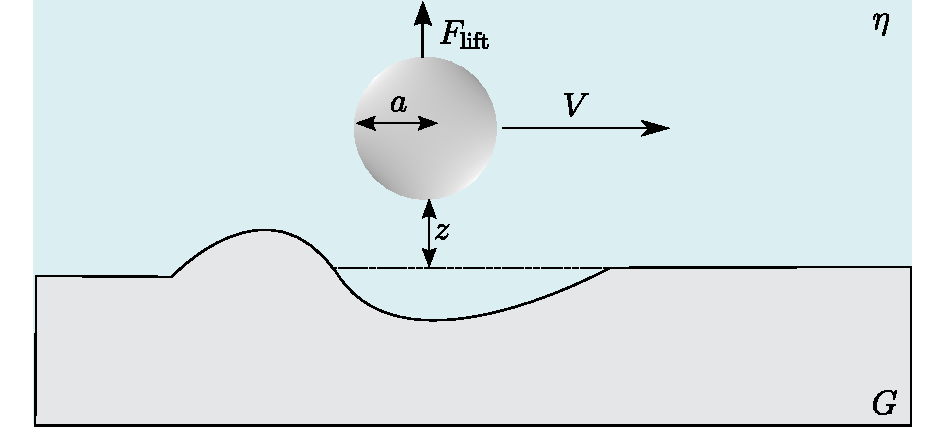
\includegraphics{02_body/chapter4/images/EHD_forces/drawing_system.pdf}
	\caption{Schema of a spherical colloid of radius $a$  immersed in a fluid of viscosity $\eta$ sliding at a velocity $V$ above an incompressible and linear-elastic substrate of shear elastic modulus $G$. From the elastohydrodynamic interactions between the particle and the soft wall arises a net lift force $F_\mathrm{lift}$ (see Eq.~(\ref{Eq.lift_deter})).}
	\label{fig.shema_EHD}
\end{figure}



Elastohydrodynamic (\gls{EHD}) is the branch in physics that permit to model the interaction between elasticity and hydrodynamic. We will here focus particularly focus to \gls{EHD} in lubrication, which permits to model the physics of sliding motion between objects with a fluid-lubricated contact. Lubrication \gls{EHD} is present in many length scales and timescales, including for example, landslides, roller bearings or blood cells motion in microfluidic devices. It is recently, in 2015, that the problem of a free particle that can sediment, slide or roll near a soft surface has been treated. As the particle slides near the surface, they moved fluid deforms the soft wall surface. One of the main results of \cite{Salez} is that sliding induced a symmetry breaking of the deformation; hence, a net force is applied to the sliding object. They further show that this force is oriented towards the particle, and, thus act as a self-sustain \gls{EHD} lift force. The first experimental proofs of this force has been done at the macro scale using negatively buoyant centimetric cylinders immersed in a viscous fluid sliding down a tilted wall that is coated with an elastic layer. They show that the self-sustained \gls{EHD} lift reduces the friction by nearly an order of magnitude and suggests that this \gls{EHD} force could partially explain phenomena such as reduced wear in animal joints and long-runout landslides. The \gls{EHD} lift force has also recently been measured at the micro-scale, using micron-sized colloidal spheres in micro channels in a shear flow. However, all of this experiment uses a system which is out of equilibrium, and, we would like to test if Brownian motion could trigger such an effect. In the soft lubrication theory, and, taking a sphere of radius $a$ moving at constant velocity $V$, in a solvent of viscosity $\eta$, at a distance $z$ for a thick (by respect to the particle radius), incompressible, linear-elastic substrate of shears elastic modulus $G$, the lift force $F_\mathrm{lift}$ reads:

\begin{equation}
	F_\mathrm{lift} \simeq \frac{\eta^2 V^2}{G} \frac{a^{5/2}}{z^{5/2}} ~.
	\label{Eq.lift_deter}
\end{equation}

To incorporate fluctuations into this deterministic picture, an idea is to replace the velocity $V$ in Eq.~(\ref{Eq.lift_deter}) by the typical Brownian velocity obtain through the Maxwell-Boltzmann distribution $\sqrt{k_\mathrm{B}T / m}$, leading the following estimate of the Brownian \gls{EHD} lift force:

\begin{equation}
	F_\mathrm{lift, Brown} \simeq \frac{\eta ^2 k_\mathrm{B}T}{G\rho_\mathrm{p} a^{1/2} z^{5/2}} ~.
	\label{Eq.lift_brown}
\end{equation}


From this equation, we can observe a counterintuitive effect, as the particle radius decreases (the surface of contact), the larger the \gls{EHD} force $F_\mathrm{lift, Brown}$ is. Taking typical biophysics value such as $G \simeq 10$ kPa, $\rho_\mathrm{p} = 1350$ kg.m$^{-3}$ and $a=100$ nm, the \gls{EHD} force reaches the picoNewton order of magnitude. The latter means that microscopic entities in biology and nanoscience may spontaneously trigger large Brownian \gls{EHD} couplings, drastically affecting their dynamics. However, it is important to note that it is a simple estimate and, contains a high risk of conceptual failure associated, for example, to the lake of compensating drift at equilibrium as we have with a hard wall (see Eq.~(\ref{Eq.spurious_drift})). To do the soft coating experimentally, we use Polydimethylsiloxane (\gls{PDMS}), as a soft surface.

\subsubsection{PDMS}

\gls{PDMS} is a silicone-based organic polymer which is widely used due to its versatility and ease of use \cite{wolf_pdms_2018}. Its chemical formula is:

\begin{equation}
	\mathrm{CH_3[Si(CH_3)_2 O]}_n \mathrm{Si(CH3)_3} ~,
\end{equation}

where $n$ is the number of $\mathrm{Si(CH_3)_2 O}$ dimethyl groups. By mixing a solution of \gls{PDMS} chains with curring agent containing, for example hydrosilane groups ($\mathrm{SiH}$), bonds, or crosslink between different \gls{PDMS} chains are appearing as shown in Fig.\ref{fig.crosslink}.




\begin{figure}[H]
	\centering
	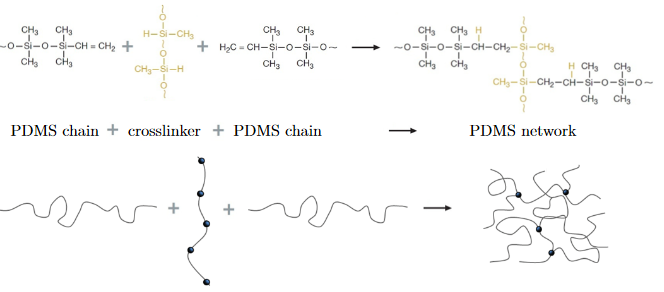
\includegraphics[scale = 0.8]{02_body/chapter4/images/EHD_forces/figure_cross.png}
	\caption{Figure taken from \cite{tucher_analysis_2016}. Examples of crosslinking reaction between the \gls{PDMS} chains and a curing agent containing hydrosilane groups.}
	\label{fig.crosslink}
\end{figure}


Due to this crosslink, the \gls{PDMS} turns into an incomprehensible and linear-elastic solid. Some of its characteristics are to be hydrophobic and to exhibit strong gas permeability \cite{xia_soft_1998}. The elasticity modulus $G$ of the crosslinked \gls{PDMS} can be tuned by changing the mixing ratio of base polymer solutions and curing agent. For example, for one of the most used \gls{PDMS} Sylgard 184, a mixing ratio of $10:1$ leads to an elastic modulus $G=1.5$ MPa and $G\simeq 100$ kPa for a $35:1$ ratio \cite{wang_crosslinking_2014}. To prepare experimental, samples, it possible to spin coat the microscope slides with base:agent mix before it is cured in order to have a thick soft surface. However, for simplicity and check if we can observe any forces with our experiment we first decided to use already prepared samples sold by Ibidi, these came as soft coated dishes with a coverslip on the bottom that we can directly fit onto our microscope.


\subsubsection{Measuring non-conservative forces}

To measure the non-conservative forces that a felt by a Brownian particle diffusing on top of a soft surface, we do the exact same experiment and data analysis as developed in the section \ref{section:expresults}. As the \gls{EHD} force do not derive from a potential, we need to extract the non-conservative forces $F_\mathrm{NC}$ at a distance of 100 nm from the wall, to do so, by combining Eqs.~(\ref{Eq.conservative_force})~and~(\ref{Eq:Force}), the non-conservative force reads:

\begin{equation}
	F_\mathrm{NC} = F_z(z) - F_z ^\mathrm{eq}(z)
\end{equation}

As seen in Fig.\ref{fig.ncforce} the measured $F_\mathrm{NC}$ for two different elastic moduli $G=15$ and $28$ kPa, only gets out of the noise for $F_\mathrm{NC} > 10$ fN, as the plot is in logarithmic scale negative values do not show. These first experiment shows that the particle seems to trigger some non-conservative forces. However, this first experiment is not sufficient to tell if it is the \gls{EHD} lift force but give some support to continue the experiment.

In the forthcoming experiment, we will vary three parameters, $\eta$, $G$ and $a$ to check if we can prove the existence of a universal plot, and show the $F_\mathrm{lift, Brown}$ correctly varies as a function of $\frac{\eta^2}{Ga^{1/2}} $ as shown in Fig.\ref{fig.ncforcenormalized} with the first experiments.

\begin{figure}[H]
	\centering
	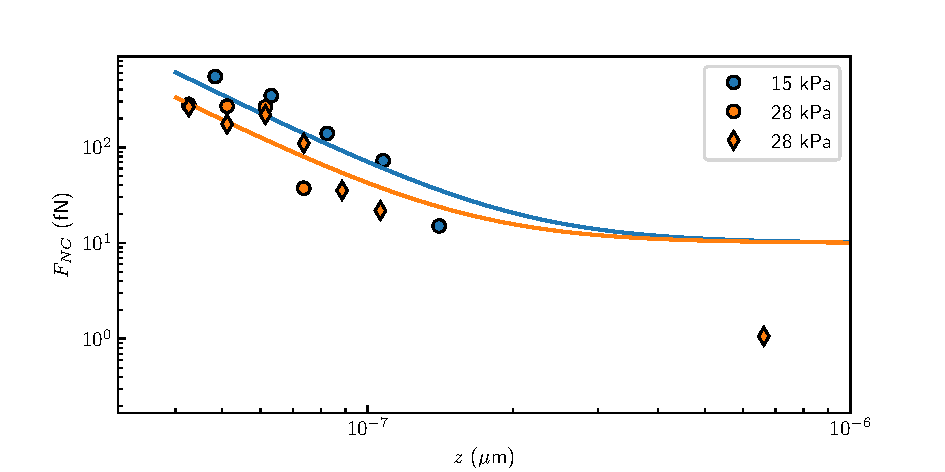
\includegraphics{02_body/chapter4/images/EHD_forces/EHD_force.pdf}
	\caption{Non-conservative forces measured experimentally for colloidal particles of radius $a=1.5 ~\mathrm{\mu m}$ diffusing above an incompressible and linear-elastic substrate of shear elastic modulus $G=15$ and $28$ kPa. Plain line corresponds to the Brownian model of the \gls{EHD} lift force $F_\mathrm{lift, Brown}$ (see Eq.~(\ref{Eq.lift_brown})) with an added noise-level of $10$ fN.}
	\label{fig.ncforce}
\end{figure}

\begin{figure}[H]
	\centering
	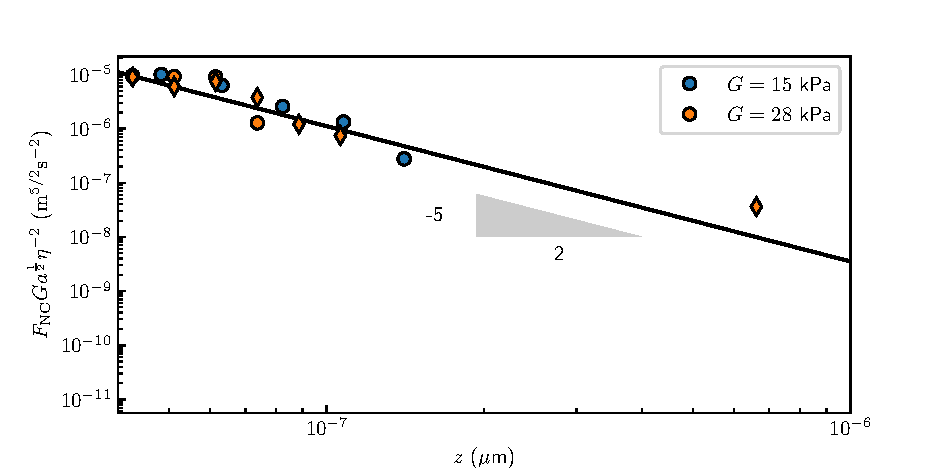
\includegraphics{02_body/chapter4/images/EHD_forces/EHD_force_rescale.pdf}
	\caption{Non-conservative forces  normalized $ G\sqrt{a} $ by measured experimentally for colloidal particles of radius $a=1.5 ~\mathrm{\mu m}$ diffusing above an incompressible and linear-elastic substrate of shear elastic modulus $G=15$ and $28$ kPa. Plain line corresponds to the Brownian model of the \gls{EHD} lift force $F_\mathrm{lift, Brown}$ (see Eq.~(\ref{Eq.lift_brown})) with an added noise-level of $10$ fN.}
	\label{fig.ncforcenormalized}
\end{figure}


\subsection{Close wall stuck motion}

\begin{figure}[H]
	\centering
	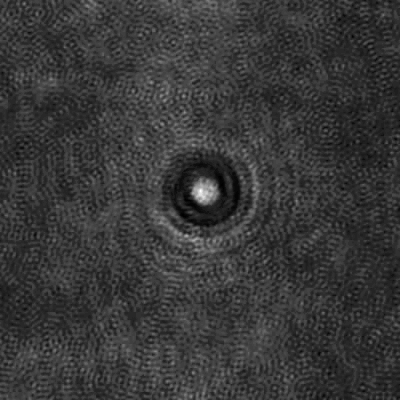
\includegraphics[scale=0.5]{02_body/chapter4/images/stucked_particle/ghost.png}
	\caption{Median image of a stuck particle. The median is calculated over $120$ images taken every $30$ s.}
	\label{fig.ghost_stucked}
\end{figure}

As we have done the experiments to measure the Debye length $\ell _\mathrm{D}$ as a function of the concentration of NaCl, we observed that some particle was stuck at the surface. As we first expected, we were not observing any movement from the stuck particle. However, surprisingly we observe that some particle was slightly diffusing. This slight diffusion can be observed directly from the raw data, by looking at the median of the video, as shown Fig.\ref{fig.ghost_stucked}, one can observe the ``ghost" of the particle due to its movement in time. Moreover, as we cannot properly have the background in this experiment since the particle do not diffuse enough, the statistical error of the tracking is increased. The measured trajectory is shown Fig.\ref{fig.trajectory_stuck}, we observe that mechanical drift happened during the experiment, this could be due to a drift of the sample or the objective, for example. This drift is of the order of magnitude of $2 ~ \mathrm{\mu m.h^{-1}}$ along the $x$- and $y$-axis and  $6 ~ \mathrm{\mu m.h^{-1}}$, in the following we look at the short time dynamics ($t < 1$~s), since the drift at this time scale is of the order of the nm it is not necessary to remove the drift from the trajectory.

\begin{figure}[H]
	\centering
	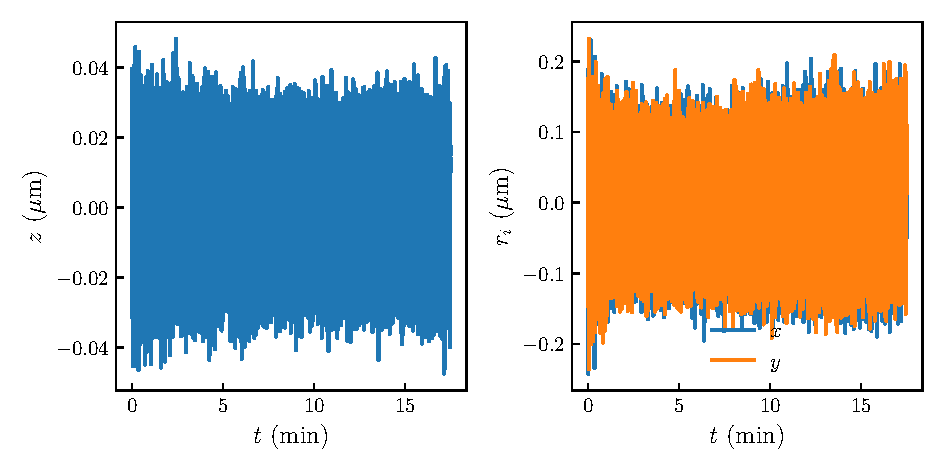
\includegraphics{02_body/chapter4/images/stucked_particle/trajectory_stucked.pdf}
	\caption{Raw trajectory measured using the Mie tracking technique for the $x$-, $y$- and $z$- axis of a particle of radius $a=1.5 ~\mathrm{\mu m}$. The time between each frame is$1/200$ s. }
	\label{fig.trajectory_stuck}
\end{figure}



Let's focus directly on the dynamics of the system, the \gls{MSD} along the $x$-, $y$- and $z$-axis is shown in Fig.\ref{fig.MSD_stucked}. We observe that the \gls{MSD} along the $z$- axis is a constant, it can be the case because it moves less that the statistical error tracking, the experiment could thus be bound by the experimental precision, or, a diffusion regime could be at a shorter time. As we here can't observe any diffusion regime on the $z$-axis, we can't determine if we are bound the tracking; hence, I will not physically comment the results obtained along the $z$-axis. However, on the $x$-axis, interestingly we can observe two regimes as had for the $z$ before meaning that the particle is diffusing in a potential which isotropic along the $x$- and $y$-axis, as if the particle was rolling on the surface due to the rugosity for example (NEED TO ASK YACINE FOR REF). The diffusive regime, at a short time, is linear with $\Delta t$ showing a normal diffusion with  average diffusion coefficients (see Eq.~(\ref{averagediff}))  $\langle{D_\parallel}\rangle= \langle D_x\rangle=\langle D_y \rangle =0.14\,D_0$. This diffusion coefficient is lower than what is obtainable using the previous defined equation of $D_\parallel$, Eq.~(\ref{Eq:etax}), which we do not explain.



\begin{figure}[H]
	\centering
	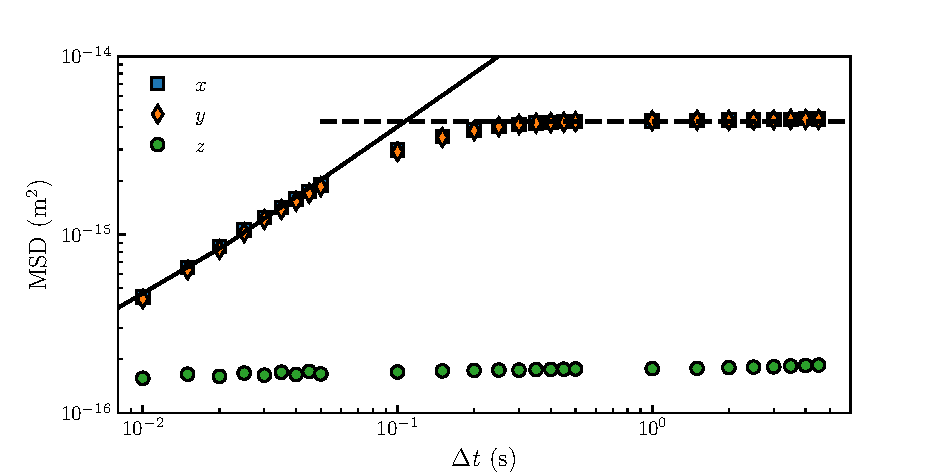
\includegraphics{02_body/chapter4/images/stucked_particle/MSD_stucked.pdf}
	\caption{Measured mean-squared displacements of a stuck particle (MSD, see Eq.~(\ref{MSDdef})) as functions of the time increment $\Delta t$, for the three spatial directions, $x$, $y$, and $z$. The solid line is the best fit to Eq.~(\ref{averagediff}), having $\langle D_i \rangle$ as a free parameter,
		providing the average diffusion coefficient $\langle{D_\parallel}\rangle= \langle D_x\rangle=\langle D_y \rangle =0.14\,D_0$. The plain gray line is the average value of the plateau of the MSD along the $x$- and $y$-axis, providing $ \lim\limits_{\Delta t \rightarrow \infty }\langle \Delta x ^2 \rangle = 4.3 \times 10 ^{-15} ~ \mathrm{m^2}$.}
	\label{fig.MSD_stucked}
\end{figure}

The plateau of the MSD along the $x$ and $y$ gives a value of  $ \lim\limits_{\Delta t \rightarrow \infty }\langle \Delta x ^2 \rangle = 4.3 \times 10 ^{-15} ~ \mathrm{m^2}$. By supposing that the particle is in a harmonic oscillator potential, we can make an estimate of the spring constant $k_\mathrm{H}$, using the relation:

\begin{equation}
	k_\mathrm{H} = \frac{k_\mathrm{B} T}{ \lim\limits_{\Delta t \rightarrow \infty }\langle \Delta x ^2 \rangle}  \simeq \frac{4 \times 10^{-21}}{4.3 \times 10 ^{-15}} \simeq 1 ~ \mathrm{\mu N . m^{-1}}~.
\end{equation}

An idea we have is to try to observe the same phenomenon using a soft surface and see if we can observe a change of $k_\mathrm{H}$ as a function of the elastic modulus $G$. If the latter assumption is possible, this experiment could lead to local determination of elastic modulus using Brownian probes. Additionally, we can look at displacement \gls{PDF} $P_i$ as shown on the Fig.\ref{fig.P_dxz_stucked}. Contrary to the result we had for a free diffusing particle (See Fig.\ref{fig.displacement}) we do not observe non-Gaussianity. Moreover, distribution $P_z$ seems to corroborate with the fact that we are bound to the fit error on the fit along the $z$-axis. Indeed, if the particle is at equilibrium, which should be the case with a MSD being constant, $P_z$ should be given by exponential as shown in Fig.\ref{fig.displacement}-e). Here $P_z$ looks like a Gaussian distribution of the fit statistical error.


\begin{figure}[H]
	\centering
	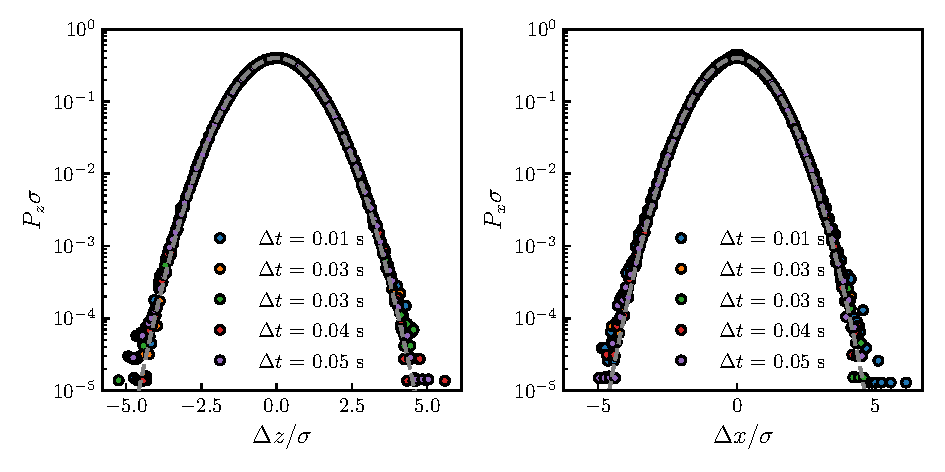
\includegraphics{02_body/chapter4/images/stucked_particle/P_xz_stucked.pdf}
	\caption{ Normalized probability density functions $P_i\,\sigma$ of the normalized displacements $\Delta x/\sigma$ and $\Delta z/\sigma$, at short times, with $\sigma^2$ the corresponding MSD (see Fig.\ref{fig.MSD_stucked}), for different time increments $\Delta t$ ranging from 0.01~s to 0.05~s, as indicated with different colors. The gray dashed lines are normalized Gaussian distributions, with zero means and unit variances.}
	\label{fig.P_dxz_stucked}
\end{figure}

\subsection{Direct relative distance measurement using Mie}

One of the effects that is not taken into account in the Mie theory presented in the section \ref{chap:LM_fit} is the presence of the glass slide. Indeed the focal plane, where the holograms are recorded is in the glass slides, thus, the holograms should be refracted at the glass interface. However, it is not a problem, for they realized fit, indeed, to have faster fit, we use only the few maxima leading to radial distance of $\simeq 5 ~\mathrm{\mu m }$ for a height $z\simeq 15~\mathrm{\mu m}$, leading to a maximal angle of incidence $\theta = \tan^{-1} (5/15) \simeq 18.5 ^{\circ} $. As we are working with small angles, we can suppose that for the first maxima, there is not refracted. 

However, the small angle approximation does not hold for higher order maxima, thus as the refraction angle depends on the wall-particle distance, adding it to the Mie theory could lead to a direct measurement of the particle height. Moreover, the Mie fitting would even more robust since a mechanical drift of the sample of the objective would not change the refractive angle of the particle. However, the main difficulty is to be able to have a more stable imaging device to detect with a high accuracy the highest order maxima which are less intense.


\begin{figure}[H]
	\centering
	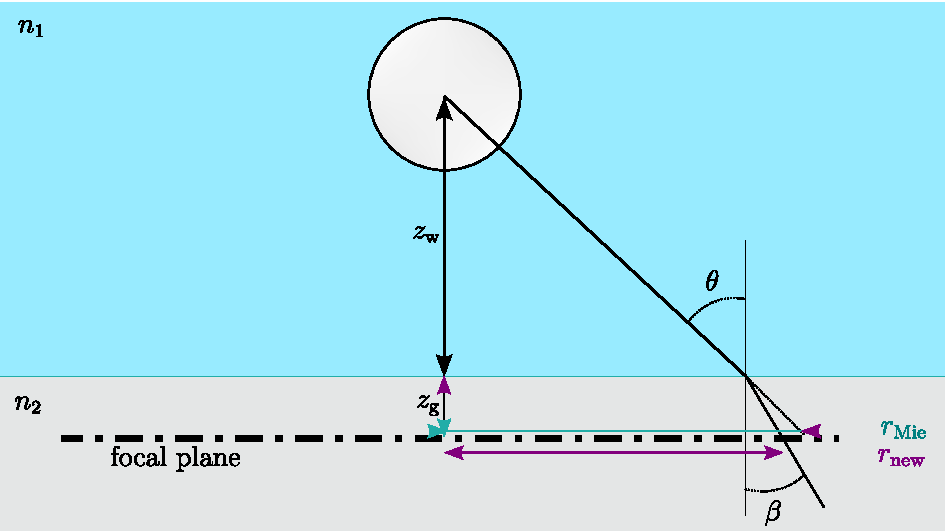
\includegraphics{02_body/chapter4/images/h_measurement/drawing_angles.pdf}
	\caption{Scheme of a particle immersed in a fluid of index $n_1$ above a glass substrate of optical index $n_2$. The particle is at a distance $z_\mathrm{w}$ above the glass subrate, and the objective focal plane $z_\mathrm{g}$ below the interface. Due to the Snell-Descartes law, light with an incident angle $\theta_1$ is refracted with an angle $\beta$. }
	\label{fig.schema_h}
\end{figure}

Let us build a simple model using the Snell-Descartes’s law to take into account the refraction at the glass interface, the system is schematized in Fig.\ref{fig.schema_h}. We decompose the height of the particle $z$ in two parts such that:

\begin{equation}
	z = z_\mathrm{w} + z_\mathrm{g} ~,
\end{equation}

where $z_\mathrm{g}$ is the interface-focal plane interface and $z_\mathrm{w}$ the interface-particle distance, the latter being the distance we want to measure. We want to write the radial intensity of the hologram $I$, taking into account the refraction, let us write  $I_\mathrm{Mie}$ the Mie solution without the refraction and $I_\mathrm{new}$ the modified theory. An incident ray coming from the particle with an angle $\theta$ is refracted with an angle $\beta$, as shown in Fig.\ref{fig.schema_h}. Using trigonometry and the Snell-Descartes's law ($n_1 \sin(\theta)  = n_2 \sin(\beta)$), those angles writes:

\begin{equation}
	\theta = \tan ^{-1} \left( \frac{r_\mathrm{Mie}}{z_\mathrm{w} + z_\mathrm{g}}\right) ~,
\end{equation} 

and,

\begin{equation}
	\beta = \sin ^{-1} \left(\frac{n_1 \sin (\theta)}{n_2}\right) ~.
\end{equation}

Without refraction, the light arrives at the focal plane at a distance $r_\mathrm{Mie}$ as shown in Fig.\ref{fig.schema_h}, due to the refraction this distance is modified to $r_\mathrm{new}$:

\begin{equation}
	r_\mathrm{new} = r_\mathrm{Mie} + z_\mathrm{g}(\tan(\beta) - \tan(\theta)) ~.
\end{equation}

Due to the change of optical path, the Mie scattering field (see Eq.~(\ref{EMie})) undergoes a phase difference $\Delta \varphi_\mathrm{w}$ in the fluid  and  $\Delta \varphi_\mathrm{g}$ in the glass substrate:

\begin{equation}
	\Delta \varphi_\mathrm{w} = \frac{2 \pi}{\lambda} n_1 z \tan(\theta ')~,
\end{equation}

and,

\begin{equation}
	\Delta \varphi_\mathrm{g} = \frac{2 \pi}{\lambda} n_2 z \tan(\beta ')~,
\end{equation}

where $\theta '$ and $\beta '$ are given by:

\begin{equation}
	\theta ' = \tan ^{-1} \left( \frac{r_\mathrm{new}}{z_\mathrm{w} + z_\mathrm{g}}\right) ~,
\end{equation}

and,

\begin{equation}
	\beta ' = \sin ^{-1} \left(\frac{n_1 \sin (\theta ')}{n_2}\right) ~.
\end{equation}

Moreover, a part of the light is reflected onto the surface, thus attenuation the scattering field by a factor $T = (n_1+n_2) / 2n_2$. Finally, taking the phase difference, the corrected scattered field $E^\mathrm{new} _s$ writes:

\begin{equation}
	E_s^\mathrm{new} = TE_s \exp(-j(\Delta \varphi_\mathrm{w} - \Delta \varphi_\mathrm{g})) ~,
\end{equation}

with the hologram normalized radial intensity given by:

\begin{equation}
	\frac{I(r)}{I_0(r)} = \frac{|E_s^\mathrm{new}(r) + E_0(r)|}{E_0(r)}
	\label{Eq.modified_mie}
\end{equation}

We worked on this project with Mathias Perrin, a specialist of the numerical simulation of Mie systems and he numerically shows that the simple correction made to correctly describes the change made by the presence of the glass slide as shown in the Fig.XX. Thus, proving that it is theoretically possible to directly fit the wall-particle distance using Mie holography tracking. However, we still not succeed on applying to the experimental data, probably due to the lack of accuracy on the higher order hologram's maxima.

\begin{figure}[H]
	\centering
	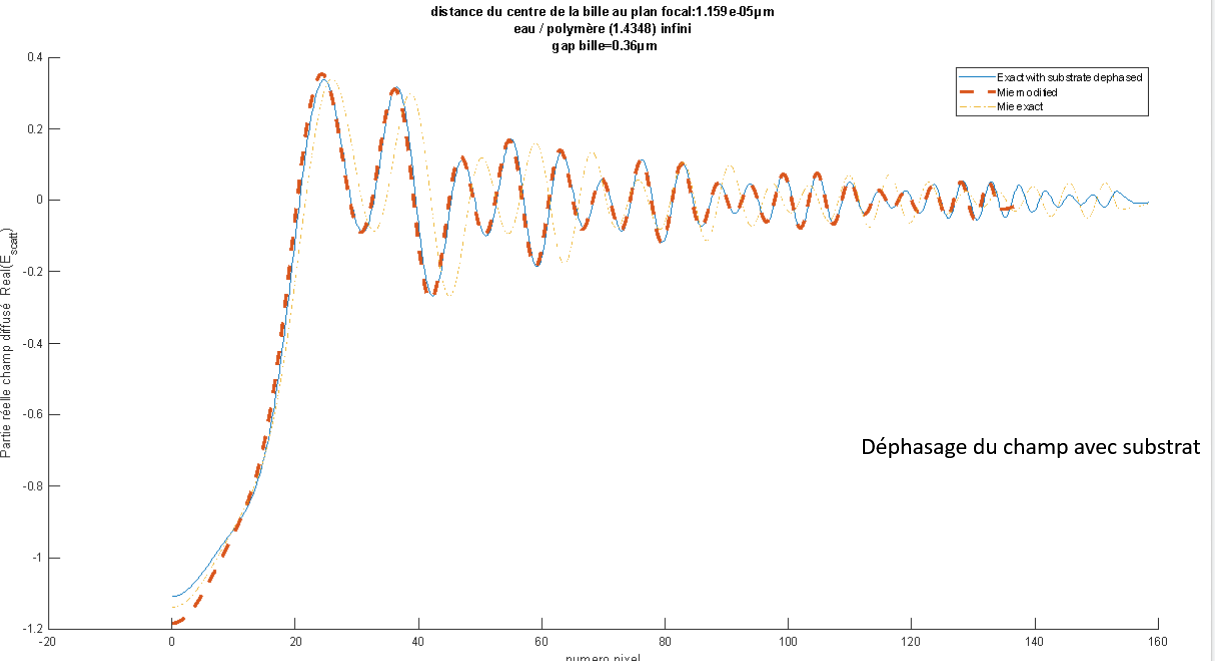
\includegraphics[scale=0.5]{02_body/chapter4/images/h_measurement/simulation_glass_correction.png}
	\caption{Numerical proof of the hologram correction due to the presence of the glass slide. The yellow dashed line represents the Mie theory without taking into account the substrate. The plain line represents the exact numerical simulation of the phase difference. The red dashed line represents the simple correction made to the Mie theory Eq.~(\ref{Eq.modified_mie})}
	\label{fig.glass_correction}
\end{figure}

\subsection{Long time 4th cumulent - Dean project}

In this subsection we consider the cumulent of higher order than 2 (\gls{MSD}). The 4th order cumulent writes:

\begin{equation}
	C_4 (\Delta t) = \frac{1}{4!} \left(
		\left\langle [ x_i(t + \Delta t) - x_i(t) ]^4 \right\rangle_t
		- 3\left\langle [ x_i(t + \Delta t) - x_i(t) ]^2 \right\rangle_t ^2
	   \right) ~.
	   \label{c4}
\end{equation}

For a Gaussian distributed variable $x$ as Brownian motion in bulk, $C_4$ is a constant as $\langle \Delta x ^2 \rangle _t ^2 = \langle x^4 \rangle_t $. Therefore, the literature often overlook the higer moments as it permits to measure and gain insights from the difference from a Gaussian distribution. However, as it has been shown along this manuscript, confined Brownian motion exhibit non-Gaussian stastical properties as shown in Fig.\ref{fig.displacement}. Thus, it could be interreseting to study the 4th cumulent of confined Brownian particles. We work on this idea with David Dean and Arthur Alexandre who are specialized in Brownian theory. Interestigly, they found interesting behaviour for the 4th cumulent for the parrallel displacement to the wall, for which the the Langevin equation is given by:

\begin{equation}
	dX_t = \sqrt{2D_\parallel(z_t)} \mathrm{d}B_t
	\label{c4.dx}
\end{equation}

After combining Eqs.~(\ref{c4})~and~(\ref{c4.dx}) and some mathematical manipulation, the 4th order cumulent writes:

\begin{equation}
	C_4(\Delta t) = \int_{-L} ^L \mathrm{d}z 
	\int ^L _{-L}\mathrm{d}z'
	D_\parallel(z) D_\parallel(z') p_0(z') 
	\sum_{\lambda > 0} \psi_{\lambda, R} (z) \psi_{\lambda, L}(z')
	\left(
	\frac{\Delta}{\lambda} - \frac{1 - \exp(-\lambda \Delta t)}{\lambda ^2},
	\right) 
	\label{c4full}
\end{equation}

where the Forward Fokker Plank as been decompsed on the set of eigenfunctions $\psi_{\lambda, R}$, the right eigenfunctions of the Generator $G$ such that:

\begin{equation}
	G\psi_{\lambda, R} = \lambda \psi_{\lambda, R} ~.
\end{equation}

For $\lambda = 0$, we have: $\psi_{0, R} = p_0$ and $\psi_{\lambda, L} = 1$. Using this decomposition, the density of probability $p$ wirtes:

\begin{equation}
	p(z, \Delta t|z') = \sum _\lambda \mathrm{e} ^{-\lambda \Delta t} \psi_{\lambda, R} (z) \psi_{\lambda, L} (z') ~.
\end{equation}

Despite the complicated form of Eq.~(\ref{c4full}) it gives nice approximations at short and long times, in the limit $\Delta \rightarrow 0$, we have:

\begin{equation}
	\lim\limits_{\Delta t \rightarrow 0 } C_4 (\Delta t) = \frac{\Delta t ^2}{2}
	\left(
	\langle D_\parallel ^2 \rangle - \langle D _\parallel \rangle ^2 
	\right)~,
\end{equation}

where the averages are done over the equilibrium distribution $P_\mathrm{eq}$ and thus vary as a function of $\Delta t ^2$ at short time. Eq.~(\ref{c4full}) can also me approximated, in the limit $\Delta t \rightarrow + \infty$ where we have:

\begin{equation}
	\lim\limits_{\Delta t \rightarrow \infty } C_4 (\Delta t) = C_4 ^0 \Delta t - C^1 _4 ~,
\end{equation}

Where $ C_4 ^0$ and $ C_4 ^1$ are constants that depends on the equilibrium distribution $P_\mathrm{eq}$, and could be written as a function of $B$, $\ell _ \mathrm{D}$, and $\ell _\mathrm{B}$. Unlike the first and second moment of the parrallel displacement,(the displacement distribution $P_x(\Delta x)$ and the \gls{MSD} $\langle \Delta x ^2 \rangle_t $ respectively), the 4th cumulent a peculiar regime when the particle reach equilibrium. This result is thus interresting as it gives a new observable of the equilibrium properties on the parallel displacement. If this theory is verified, it could be added to our inference method (see section \ref{section:expresults}) in order to gain precision and robustess.

As we are only interested to the $x$- and $y$-axis displacement to show this result, we do not need 3D tracking. Thus, we only need to find the holograms centroid, and therefor use faster algorithm than the Mie framework. To do so we use the Trackpy package \href{https://github.com/soft-matter/trackpy}{\faGithub} \cite{allan_soft-mattertrackpy_2021} which implements the Crocker–Grier algorithm \cite{crocker_methods_1996} which permits to track the centroid of hundred of colloids quite rapidly, as shown in Fig.XX.

From the data retrieve, we can compute the 4th cumulent using Eq.~(\ref{c4}) and we do observe a linear regime at long time as shown in Fig.XX. However, this experiment as only been done once, it is thus preliminary results that encourage continuing in this way.

\subsection{Sample ageing}

Doing the experiment on the soft surfaces, we observed that the images was becoming blurry with time, as a diffusive layer was added in the microscope's optical path. An example is shown in Fig.XX where we can see microscope images separated by three hours.


Trying to find the origin of this effect, we focused on the interface between the soft PDMS layer and glass. Doing so we observe a structure that looks like bubbles, as shown in Fig.XX. We observe that this effect happens faster as the PDMS is softer (lower modulus) and the bubble seems to be also bigger, as shown in Fig.XX. One of the idea we have to explain this phenomenon comes from the high gas permeability of PDMS that could lead to a gas accumulation between the PDMS and glass. The origin of this gas would come from the naturally present gas inside the colloid suspension.
